\section{Основные понятия}

\begin{table}[h!]
    \caption{Спецсимволы}
    \label{specsymbols}
    \begin{tabular}{|l|p{0.75\textwidth}|}
        \hline
        \textbf{Спецсимвол} &
        \textbf{Значение} \\ \hline

        \verb|~| & "<неразрывный пробел"> \\ \hline
        \verb|#| & TODO: что это? \\ \hline
        \verb|$| & математическое окружение \\ \hline
        \verb|^| & верхний индекс или показатель степени (в математическом окружении) \\ \hline
        \verb|_| & нижний индекс (в математическом окружении) \\ \hline
        \verb|%| & начало комментария; заканчивается комментарий на конце строки \\ \hline
        \verb|{ }| & группа \\ \hline
    \end{tabular}
\end{table}

\bigskip

\noindent
В пакете \textbf{babel} кавычки являются спецсимволом.

\begin{table}[h!]
    \caption{Кавычки в пакете babel}
    \label{quotes_in_babel}
    \begin{tabular}{|l|l|p{0.7\textwidth}|}
        \hline
        \textbf{LATEX} &
        \textbf{OUT}   &
        \textbf{Описание} \\ \hline
        \verb|"<| & "< & левая ёлочка  \\ \hline
        \verb|">| & "< & правая ёлочка \\ \hline
        \verb|"`| & "` & открывающая лапка (обратный апостроф) \\ \hline
        \verb|"'| & "' & закрывающая лапка (прямой апостроф)   \\ \hline
    \end{tabular}
\end{table}

\textbf{Пробелы.} В непрерывной последовательности пробелов и знаков табуляции пробел будет печататься только один раз.

\begin{table*}[h!]
    \begin{tabular}{|l|p{0.7\textwidth}|}
        \hline
        \verb|\,| & "<неразрывный пробел"> уменьшенного размера.\\
        \hline
    \end{tabular}
\end{table*}

\textbf{Конец строки.} LATEX в непрерывной последовательности символов конца строки два символа конца строки означают переход к новому абзацу. Остальные символы конца строки игнорируются.

\begin{table*}[h!]
    \begin{tabular}{|l|p{0.7\textwidth}|}
        \hline
        \verb|\\| & конец строки в выходном файле\\
        \hline
    \end{tabular}
\end{table*}

\begin{table}[h!]
    \caption{Дефисы и тире}
    \begin{tabular}{|l|l|p{0.65\textwidth}|}
        \hline
        \textbf{LATEXT} &
        \textbf{OUT}    &
        \textbf{Описание} \\ \hline
        \verb|-| & - & кусочно-непрерывное \\ \hline
        \verb|--| & -- & краткое тире от--до (например, дорого отнимает тридцать--сорок минут) \\ \hline
        \verb|---| & --- & длинное тире --- знак препинания \\ \hline
    \end{tabular}
\end{table}

\deff{Команда --- это специальная инструкция по отображению контента в выходном файле.}\\

Синтаксис:
\begin{verbatim}
    \command
\end{verbatim}

\begin{verbatim}
    \command{argument}
\end{verbatim}

\begin{verbatim}
    \command[optional argument]{argument}
\end{verbatim}

\begin{figure}[h]
    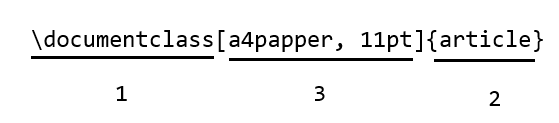
\includegraphics{fig/input_sequence_for_help.png}
    \caption{Порядок ввода текста с для активации подсказок в TexStudio}
\end{figure}


\clearpage